\chapter{Caractérisation de l'adsorption d'interface} \label{absorption}
Comme expliqué précédemment la méthode champ de phase et une méthode de capture d'interface, ainsi dans notre cas l'interface est résolue implicitement au travers des profils de concentrations. Finalement, notre système possède autant d'interfaces que de champs capturés ($n-1$ interfaces pour $n$ composants). Les interfaces peuvent alors avoir des positions différentes créant une adsorption d'interface \cite{rasolofomanana_diffuse-interface_2022}. En effet, ce décalage de position d'interface peut créer un excès de masse dans la zone d'interface. Cet excès peut alors être la cause d'une non monotonie du profil de masse volumique, induisant des instabilités de Rayleigh Taylor purement numérique.
\begin{figure}[H]
	\centering
	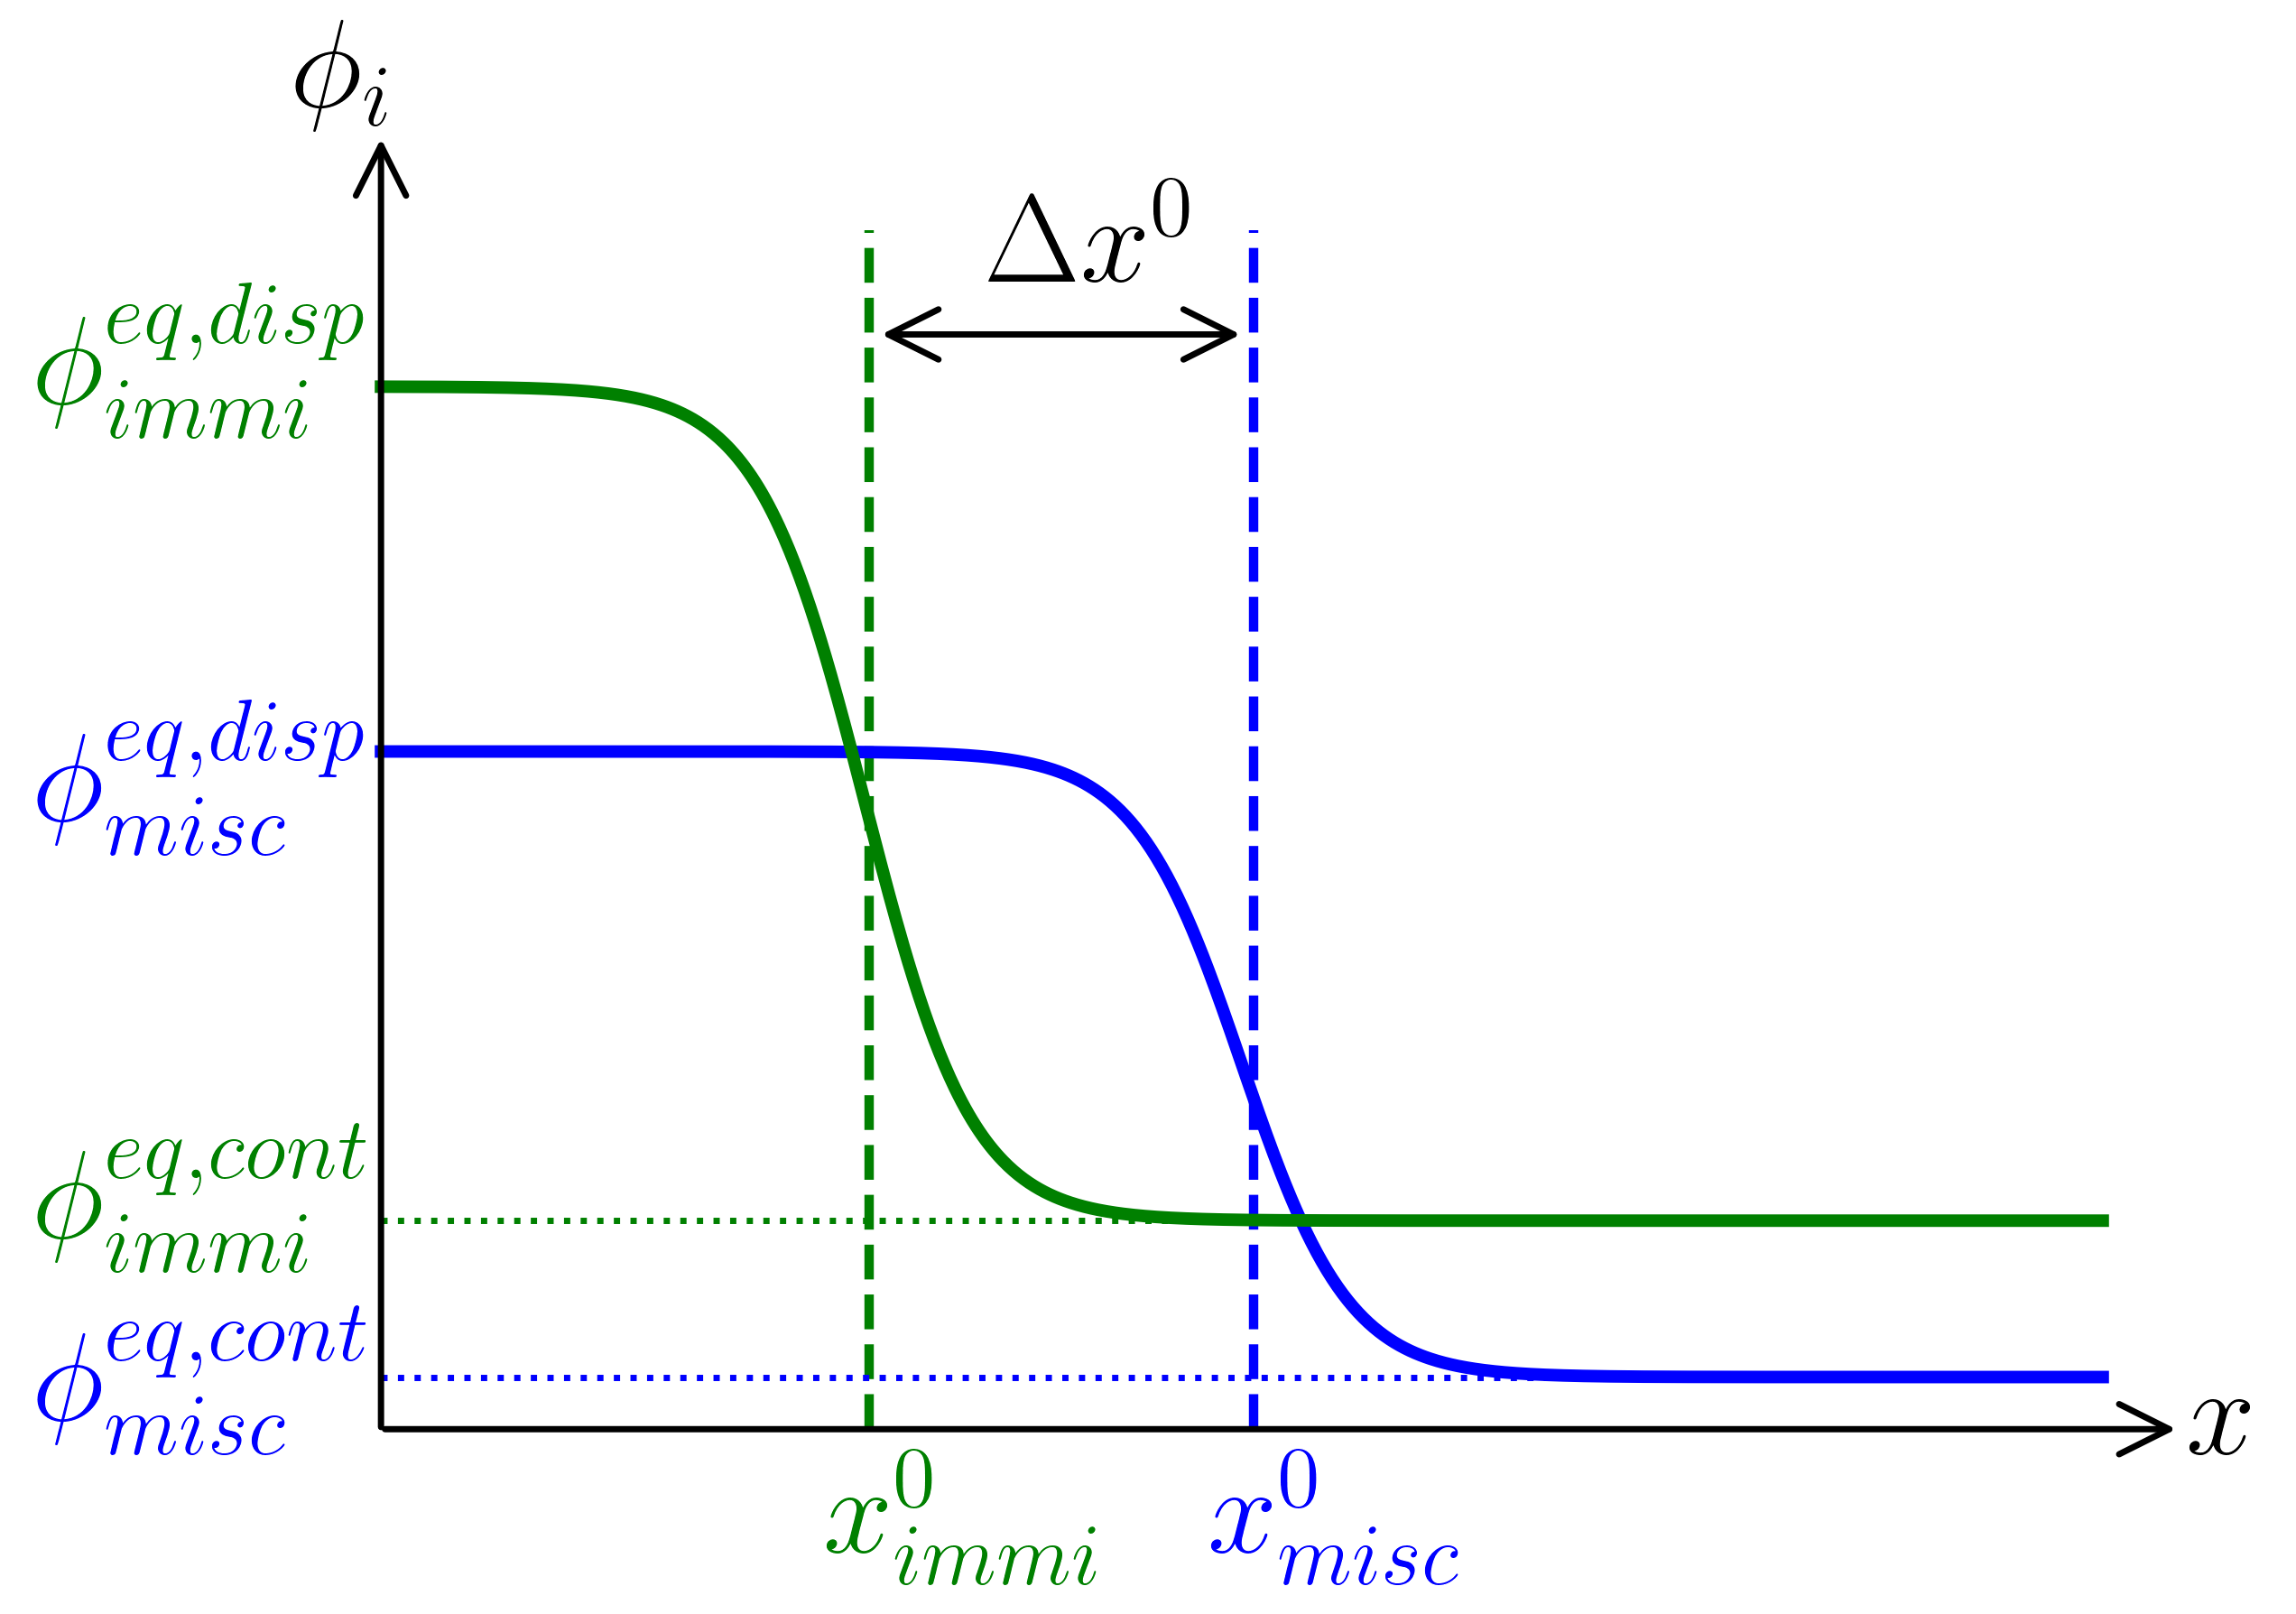
\includegraphics[width=0.5\linewidth]{figure/fig_absorption}
	\caption{Schéma représentatif de la différence de position dans un cas ternaire}
	\label{fig:figabsorption}
\end{figure}
Dans cette section nous allons donc essayer d'observer l'influence du paramétrage sur cette absorption d'interface. Dans un premier temps, nous allons caractériser l'influence de l'épaisseur d'interface $\epsilon$. Pour cela, nous faisons varier cette épaisseur, les résultats sont présentés en figure \ref{fig:planeimmiscible}.
\begin{figure}[H]
	\centering
	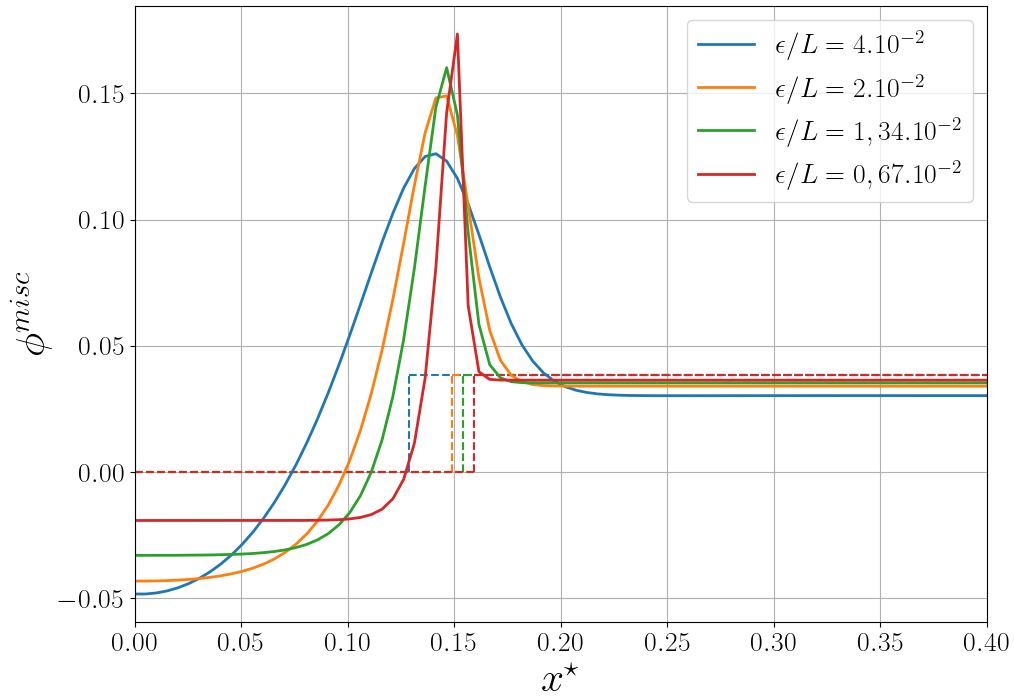
\includegraphics[width=0.6\linewidth]{figure/plane_immiscible}
	\caption{Profil d'interface du composant miscible pour différentes épaisseur d'interface $\epsilon$, les lignes en pointillés représentent les concentrations à l'équilibre dans chaque phase et les positions d'interfaces}
	\label{fig:planeimmiscible}
\end{figure}
L'interface étant non monotone, la position de l'interface miscible est obtenue en considérant la phase dispersée comme la zone où la concentration moyenne de composé miscible est nulle. L'interface immiscible est quant à elle obtenue en considérant la phase continue comme la zone où la concentration de composant immiscible est nulle :
%\begin{subequations}
%	\label{eq:all}
%	\begin{empheq}[left={\empheqlbrace\,}]{align}
%	&x^0_{misc} = x_i \mid \cfrac{x_i}{L_x}\phi_{misc}^{drop,eq}  +  \cfrac{L_x - x_i}{L_x}\phi_{misc}^{cont,eq} = \bar{\phi}_{misc}^{eq}\\
%	&x^0_{immi} = x_i \mid \cfrac{x_i}{L_x}\phi_{immi}^{drop,eq}  +  \cfrac{L_x - x_i}{L_x}\phi_{immi}^{cont,eq} = \bar{\phi}_{immi}^{eq}\\
%	& \Delta x^0 = x^0_{misc} - x^0_{immi}
%	\end{empheq}
%\end{subequations}
\begin{subequations}
	\begin{empheq}[left={\empheqlbrace\,}]{align}
	&x^0_{misc} = x_i \mid \frac{1}{x_i}\int_0^{x_i}\phi_{misc} dx = 0\\
	&x^0_{immi}= x_i \mid \frac{1}{L_x - x_i}\int_{L_x}^{x_i}\phi_{immi} dx = 0\\
	& \Delta x^0 = x^0_{misc} - x^0_{immi}
	\end{empheq}
\end{subequations}
Avec $x^0_{misc}$ (resp. $x^0_{immi}$) la position de l'interface du composant miscible (resp. immiscible) et $\Delta x^0$ l'absorption d'interface
Finalement on présente les valeurs de décalage d'interface en fonction de $\epsilon$ : 
\begin{center}
	\begin{tabular}{|c||c|c|c|c|}
		\hline 
		$\epsilon/L_x$ & $4.10^{-2}$ & $2.10^{-2}$ & $1,34.10^{-2}$ & $0,67.10^{-2}$ \\ 
		\hline 
		$\Delta x^0 /L_x$ & 0.071 & 0.035 & 0.020 & -0.020 \\ 
		\hline 
	\end{tabular} 
\end{center}

Par construction les coefficients de gradient ont un impact direct sur le profil d'interface, l'article \cite{rasolofomanana_diffuse-interface_2022} présente un paramétrisation de la matrice des coefficients de gradient pour traiter les non monotonie d'interface. Cette paramétrisation utilise la propriété de symétrie de la matrice des coefficients de gradient pour la réécrire sous la forme :
\begin{equation}
\bar{\bar{\bm{\kappa}}} = \alpha \bm{R}\bm{D}\bm{R}^T
\label{eq:param_kappa}
\end{equation}
avec : $\bm{R}$ une matrice de rotation et $\bm{D}$ une matrice diagonale de la forme :
\begin{equation}
\bm{R} =    \begin{pmatrix} 
\cos\varphi & -\sin\varphi \\ 
\sin\varphi				&  \cos\varphi
\end{pmatrix}
\end{equation}
\begin{equation}
	\bm{D}(d) =    \begin{pmatrix} 
	2 & 0 \\ 
	0 & d
	\end{pmatrix} 
\end{equation}
La cohérence avec le système binaire est assurée par le coefficient $\alpha$ obtenu tel que :
\begin{equation}
\alpha = \frac{\kappa^{bin}}{2\cos^2\varphi + d \sin^2\varphi}
\end{equation}
Les résultats de la paramétrisation de l'interface sont présentés en figure \ref{fig:profinterfacekappa}, on y observe effectivement un impact du choix de la matrice de coefficient de gradient sur le profil d'interface en régime stationnaire. Cependant, on remarque également qu'il est difficilement imaginable de complètement "lissé" notre interface à l'aide de cette méthode. De plus il est possible d'observer que la réduction de la non-monotonie s'accompagne d'un élargissement important de l'interface.
\begin{figure}[H]
		\centering
		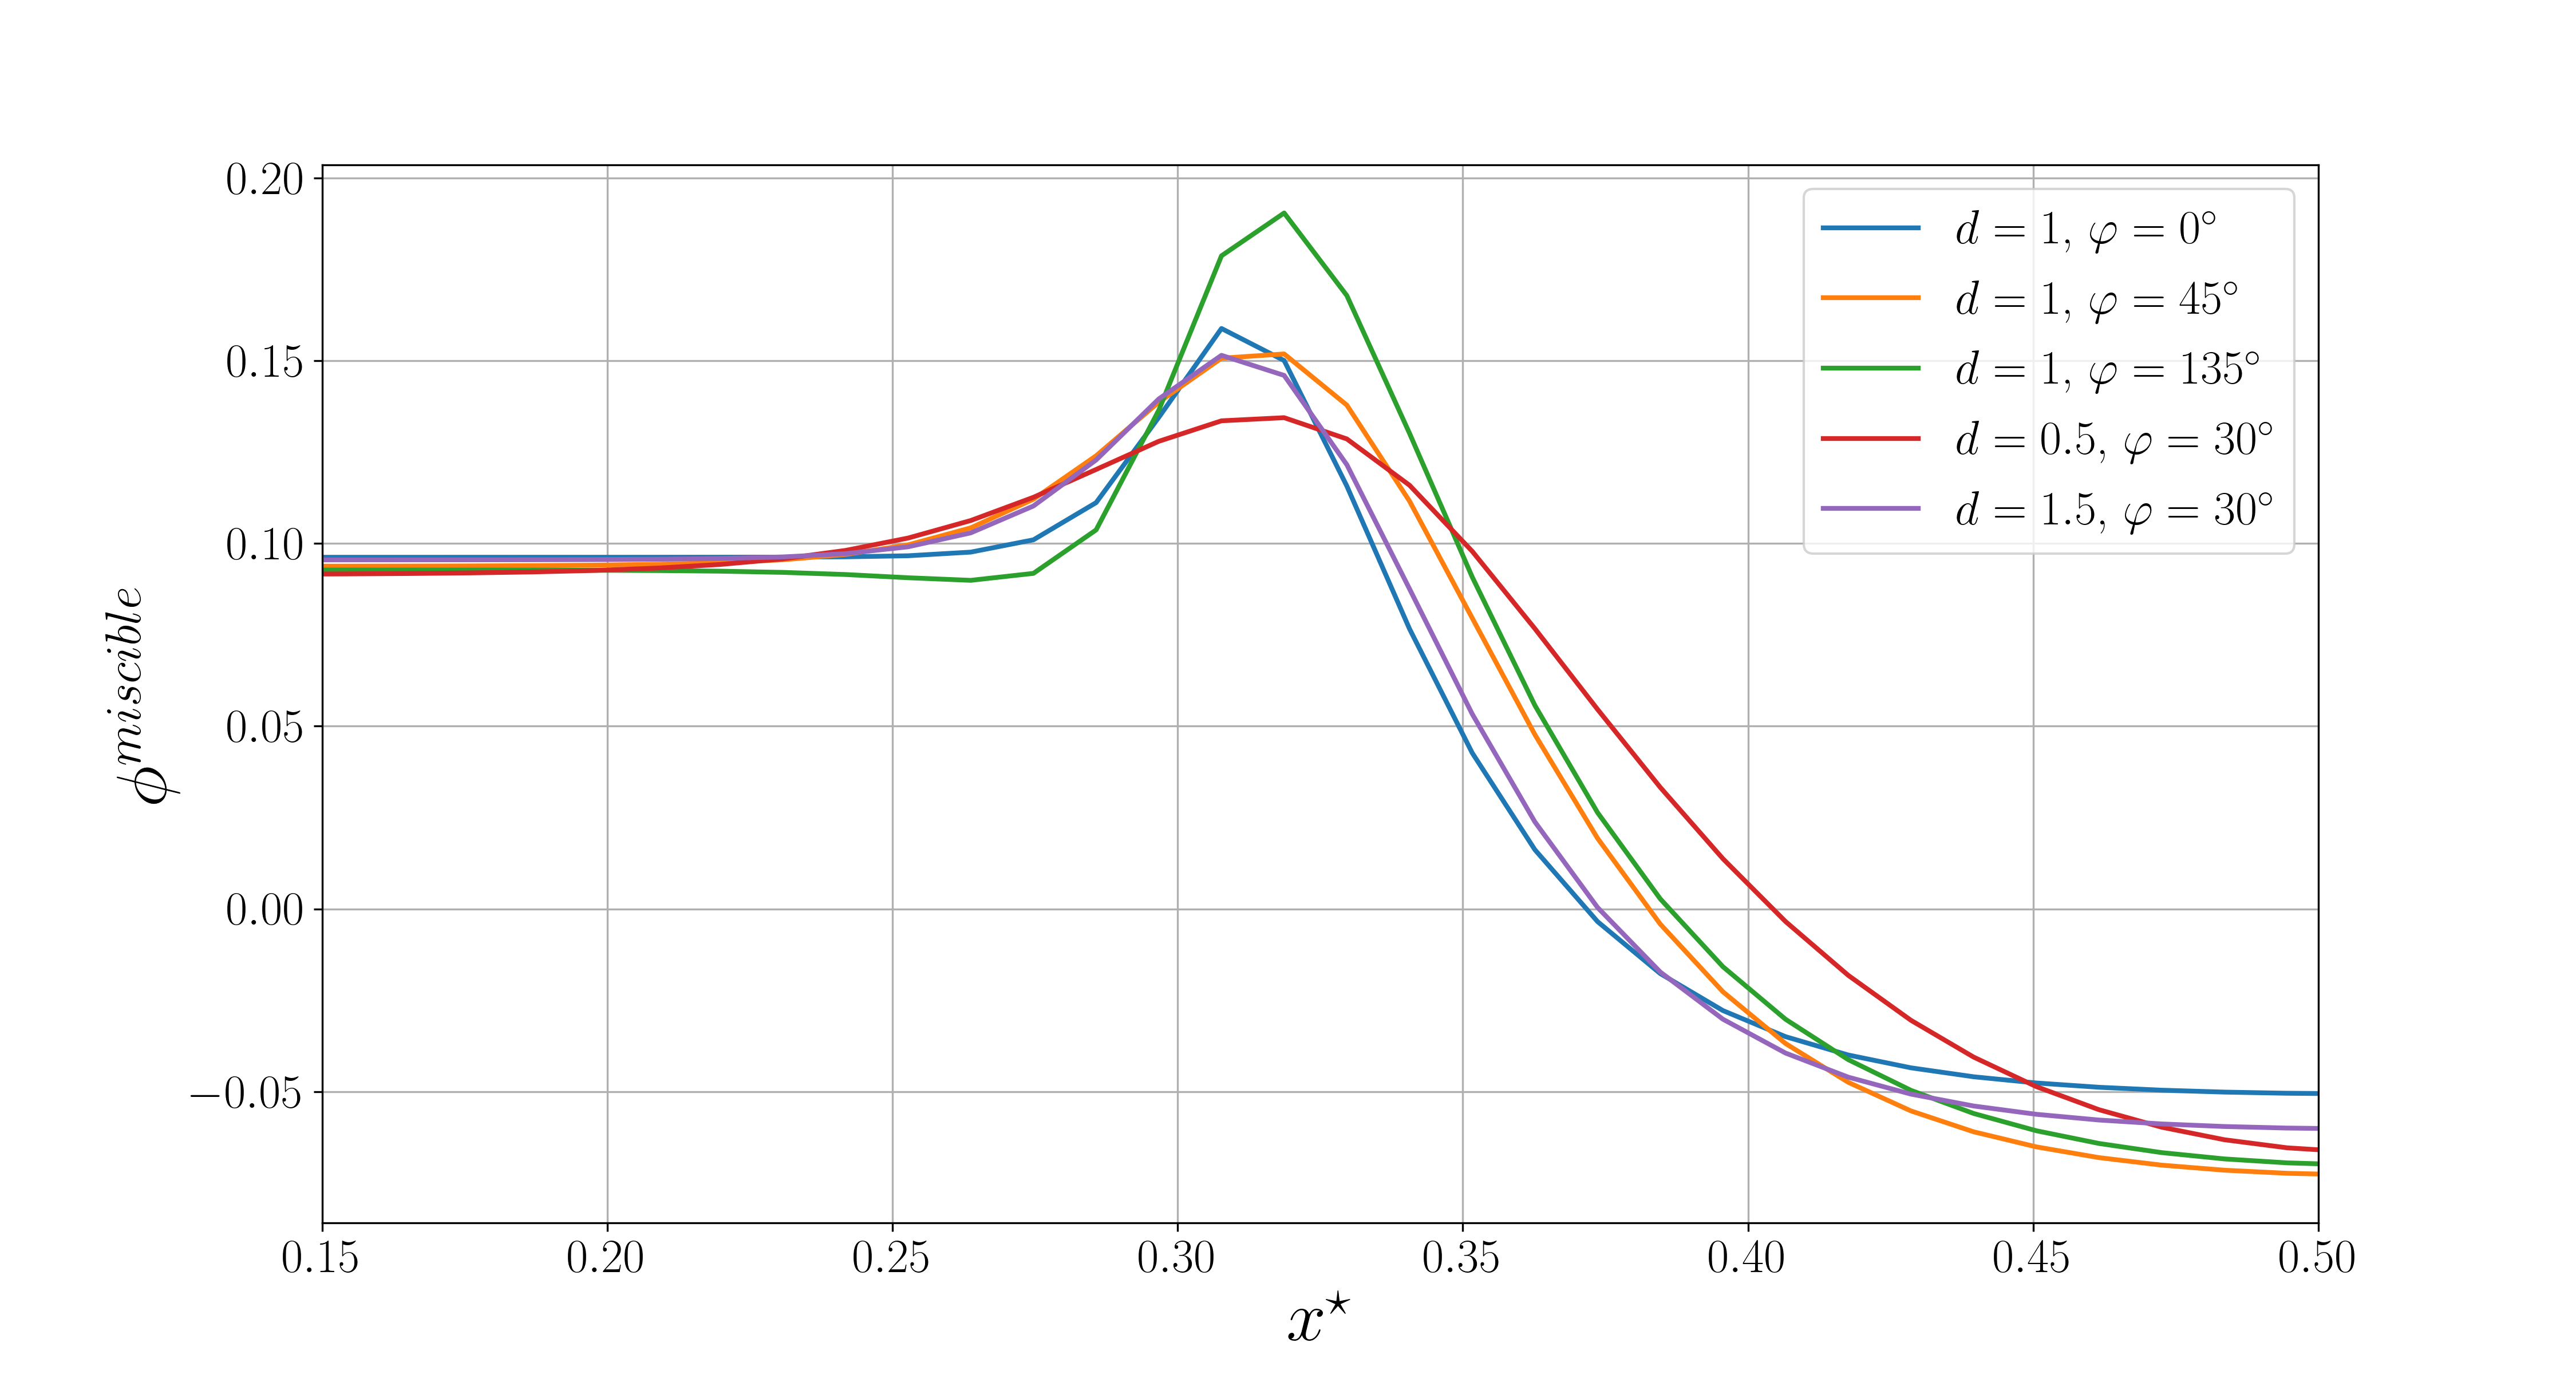
\includegraphics[width=0.7\textwidth]{figure/ProfInterfStatio2.png}
		\caption{Profils de l'interface pour différents paramétrages du coefficient de gradient}
		\label{fig:profinterfacekappa}
\end{figure}
